\documentclass[11pt]{article}
\usepackage{algorithm2e}
\usepackage[bottom]{footmisc} 
\usepackage[italian]{babel}
\usepackage[document]{ragged2e}
\usepackage{tabularx}
\justifying
\usepackage{amsfonts, amssymb, amsmath}
\usepackage{cancel}
\usepackage{float}
\usepackage{mathtools}
\usepackage[margin=2cm]{geometry}
% \setcounter{secnumdepth}{0}
\usepackage{hyperref}
\hypersetup{
    colorlinks,
    citecolor=black,
    filecolor=black,
    linkcolor=black,
    urlcolor=black
}
\usepackage{array}
\usepackage{makecell}
\usepackage{hyperref}
\usepackage[noabbrev,capitalize,italian]{cleveref}
\newcommand{\fref}[1]{\hyperref[#1]{\cref{#1}}}
\usepackage{makecell}
\usepackage{etoolbox}
\patchcmd{\thebibliography}{\section*{\refname}}{}{}{}
\usepackage{enumitem}

\usepackage{xcolor,listings}
\usepackage{textcomp}
\usepackage{color}

\definecolor{sql_comment}{HTML}{50b300}
\definecolor{sql_keywork}{HTML}{0081bd}
\definecolor{sql_string}{HTML}{b03602}
\lstdefinestyle{sqlstyle}{
    commentstyle=\color{sql_comment},
    keywordstyle=\color{sql_keywork},
    stringstyle=\color{sql_string},
    basicstyle=\footnotesize\ttfamily,
    breakatwhitespace=false,
    breaklines=true,
    keepspaces=true,
    showstringspaces=false,
    showspaces=false,
    showtabs=false
}
\lstset{style=sqlstyle}

\tolerance=1
\emergencystretch=\maxdimen
\hyphenpenalty=10000
\hbadness=10000

\begin{document}
\begin{titlepage}
    \begin{center}
        \vspace*{1.5cm}
            
        \Huge
        \textbf{Campionato di\\gare automobilistiche}
            
        \vspace{0.3cm}
        \LARGE
        Report\\[0.2em]

        \vspace{1.5cm}
          
        \begin{minipage}[t]{0.47\textwidth}
            \begin{center}
                \parbox{65mm}{\centering\large {\bf Cheikh Ibrahim $\cdot$ Zaid} \\[0.3em] Matricola: \texttt{0000974909} \\[0.3em] \href{mailto:zaid.cheikhibrahim@studio.unibo.it}{\textit{zaid.cheikhibrahim@studio.unibo.it}}} \\[2em]
            \end{center}
		\end{minipage}
		\hfill
		\begin{minipage}[t]{0.47\textwidth}\raggedleft
            \begin{center}
                \parbox{65mm}{\centering\large {\bf Xia $\cdot$ Tian Cheng} \\[0.3em] Matricola: \texttt{0000975129} \\[0.3em] \href{mailto:tiancheng.xia@studio.unibo.it}{\textit{tiancheng.xia@studio.unibo.it}}} \\[2em]
            \end{center}
		\end{minipage}  
            
        \vspace{9cm}
            
        Anno accademico\\
        $2022 - 2023$
            
        \vspace{0.8cm}
            
            
        \Large
        Corso di Basi di dati\\
        Alma Mater Studiorum $\cdot$ Università di Bologna\\
            
    \end{center}
\end{titlepage}
\pagebreak


\tableofcontents
\newpage


\section{Analisi dei requisiti}
\subsection{Requisiti espressi in linguaggio naturale}
Si vuole realizzare un database per gestire un campionato di gare automobilistiche. \\
È necessario codificare le gare, le piste su cui si svolgono, i dati relativi ai giri, eventuali infrazioni e i dati sui pit stop. \\
Inoltre, si vogliono memorizzare i dati dei piloti che partecipano e i contratti (presenti e passati) che stipulano con le scuderie. Oltre ai dati relativi alle scuderie, è richiesto registrarne le auto e i meccanici. \\
Infine, si vuole tenere traccia dei controlli di regolarità effettuati dai supervisori (della società che organizza il campionato) e dei dati degli sponsor delle gare e delle singole scuderie. \\[1em]

\subsection{Glossario dei termini}
\begin{tabularx}{\linewidth}{
        |>{\hsize=0.6\hsize}X|% 10% of 4\hsize 
        >{\hsize=1.8\hsize}X|% 30% of 4\hsize
        >{\hsize=0.6\hsize}X|% 30% of 4\hsize 
        >{\hsize=1.0\hsize}X|% 30% of 4\hsize
           % sum=4.0\hsize for 4 columns
    }
    \hline
    \textbf{Termine} & \textbf{Descrizione} & \textbf{Sinonimi} & \textbf{Collegamenti} \\
    \hline
    Società organizzante & Azienda che organizza un campionato & - & Campionato \\
    \hline
    Campionato & Numero definito di gare con classifica & - & Gare \\
    \hline
    Gare & Competizione in cui partecipa un numero fissato di piloti che effettuano un numero definito di giri di pista sul proprio veicolo & Competizione & Piste, giri, piloti, scuderie, sponsor \\
    \hline
    Giri & Percorrenza intera di una pista effettuata da un pilota & - & Piloti, gare, veicoli, pit stop, infrazioni \\
    \hline
    Piste & Località asfaltata idonea al passaggio di veicoli ad elevata velocità & - & Gare \\
    \hline
    Infrazioni & Eventi irregolari accaduti durante una gara & - & Penalità \\
    \hline
    Penalità & Tempo ulteriore assegnato come malus al tempo totale & - & Infrazioni, giri, piloti \\
    \hline
    Veicoli & Autoveicolo ad elevata velocità & Auto & Scuderie, contratti \\
    \hline
    Piloti & Persona che guida un veicolo ad elevata velocità & - & Contratti, gare \\
    \hline
    Scuderie & Azienda proprietaria di veicoli & - & Sponsor, contratti, meccanici, veicoli \\
    \hline
    Meccanici & Impiegati delle scuderie adibiti alla manutenzione dell'auto & - & Scuderie, pit stop \\
    \hline
    Supervisori & Impiegati della società organizzante adibiti ai controlli di regolarità & - & Controlli, società organizzante \\
    \hline
    Controlli di regolarità & Controlli effettuati dalla società organizzante per garantire la regolarità dei veicoli & Controlli & Supervisori, veicoli \\
    \hline
    Sponsor & Azienda che investe per apparire in gare e/o in scuderie & - & Gare, scuderie \\
    \hline
    Pit stop & Fase di un giro in cui l'auto sosta in un'apposita area di pista dove i meccanici effettuano operazioni all'auto & Box & Giri, piloti, meccanici \\
    \hline
    Contratto & Accordo stipulato tra un pilota e una scuderia per gareggiare in un campionato & - & Piloti, scuderie, veicoli \\
    \hline
\end{tabularx}

% \subsection{Eliminazione delle ambiguità presenti}
\subsection{Strutturazione dei requisiti}

\subsubsection*{Frasi relative alle gare}
Per le gare si vuole memorizzare il nome, la data di svolgimento, la pista su cui si corre, il numero di giri previsti, i piloti partecipanti e l'eventuale sponsor.

\subsubsection*{Frasi relative alle piste}
Per le piste si vogliono rappresentare il nome, la nazione e la città di collocazione, la lunghezza (in metri) e numero di posti a sedere per gli spettatori.

\subsubsection*{Frasi relative ai giri}
Per i giri si vogliono salvare il tempo impiegato (in millisecondi), il numero del giro, la gara di appartenenza e il pilota che effettua il giro.

\subsubsection*{Frasi relative alle infrazioni}
Per le infrazioni si vogliono gestire i dati riguardanti il nome e la descrizione e vengono assegnate ad un giro di un pilota sottoforma di penalità (in millisecondi).

\subsubsection*{Frasi relative ai pit stop}
Per i pit stop si vogliono rappresentare il tempo delle operazioni (in millisecondi), il tempo complessivo (tempo di entrata e uscita + tempo delle operazioni, in millisecondi), 
il giro in cui il pilota viene chiamato ai box e i meccanici che effettuano le operazioni.

\subsubsection*{Frasi relative ai piloti}
Per i piloti si vogliono memorizzare il codice fiscale, nome, cognome, luogo e data di nascita.

\subsubsection*{Frasi relative ai contratti}
Per i contratti si vogliono rappresentare il numero identificativo, il pilota ed il suo numero identificativo, la scuderia, 
la data d'inizio e di fine e l'auto assegnata.

\subsubsection*{Frasi relative alle scuderie}
Per le scuderie si vogliono gestire i dati riguardo la ragione sociale, la nazione della sede principale, l'anno di fondazione, il colore caratterizzante e i vari sponsor.

\subsubsection*{Frasi relative ai veicoli}
Per i veicoli si vogliono salvare la potenza (in cavalli), velocità massima raggiungibile, la scuderia di appartenenza e il nome del telaio.

\subsubsection*{Frasi relative ai meccanici}
Per i meccanici si vogliono memorizzare il codice fiscale, nome, cognome, luogo, data di nascita, il ruolo e la scuderia di appartenenza.

\subsubsection*{Frasi relative ai controlli}
Per i controlli di regolarità si vogliono tracciare i dati riguardo la data e l'ora, l'auto coinvolta, il supervisore e l'esito.

\subsubsection*{Frasi relative ai supervisori}
Per i supervisori si vogliono memorizzare il codice fiscale, nome, cognome, luogo, data di nascita.

\subsubsection*{Frasi relative agli sponsor}
Per gli sponsor si vogliono salvare la ragione sociale, la tipologia di azienda e la nazione della sede principale.


\subsection{Specifiche operazioni}
\begin{enumerate}
    \item Inserire una nuova scuderia (in media 1 volta ogni cinque anni)
    \item Inserire una nuova gara (in media 1 volta all'anno)
    \item Inserire il tempo di un giro del pilota sulla pista ($\sim$1000 volte per gara)
    \item Inserire il tempo pit stop ($\sim$20-60 volte per gara)
    \item Inserire un nuovo contratto tra pilota e scuderia (poche volte ogni anno)
    \item Incrementare la potenza e la velocità massima dei veicoli di una data scuderia (in media 2 volte all'anno)
    \item Visualizzare la lunghezza media, massima e minima delle piste (1 volta all'anno)
    \item Visualizzare lo sponsor di una gara (1 volta per gara)
    \item Visualizzare lo sponsor più presente (1 volta all'anno)
    \item Visualizzare la scuderia con cui un pilota ha un contratto in una determinata data (2 volte all'anno)
    \item Visualizzare nome, cognome e numero di gara dei piloti di una data scuderia con contratto attivo al momento attuale (2 volte all'anno)
    \item Visualizzare i piloti e la scuderia con cui gareggiano per una data gara raggruppandoli per scuderia (3 volte per gara)
    \item Visualizzare il tempo reale di un giro ($\sim$1000 volte per gara)
    \item Visualizzare il pilota con il tempo migliore su una data pista (1 volta per gara)
    \item Visualizzare la classifica (finale o temporanea) di una data gara ($\sim$50 volte per gara)
    \item Visualizzare i vincitori di una gara (1 volta per gara)
    \item Visualizzare in ordine decrescente i piloti e il loro numero di vittorie (1 volta per gara)
    \item Visualizzare il pilota più giovane ad aver vinto almeno una gara (1 volta per gara)
    \item Visualizzare pilota e scuderia con il pitstop più veloce (1 volta per gara)
    \item Visualizzare il supervisore che ha effettuato il maggior numero di controlli con esito negativo (poche volte all'anno)
    \item Visualizzare la scuderia e l'auto che ha avuto il maggior numero di controlli con esito negativo (poche volte all'anno)
\end{enumerate}

\section{Progettazione concettuale}
È stato seguito un approccio bottom-up per identificare i macro-argomenti.\\
Sono quindi state individuate le seguenti categorie:
\begin{itemize}
    \item Persone
    \item Aziende
    \item Partecipanti: cattura i concetti relativi alle scuderie e ai piloti.
    \item Competizione: cattura i concetti relativi allo svolgimento della gara.
\end{itemize}

\subsection{Definizioni delle entità generalizzabili}
Le entità generalizzabili sono le persone e le aziende.
\subsubsection{Definizioni delle persone}
Come persone, sono state identificate le entità supervisori, piloti e meccanici. 
\begin{figure}[H]
    \centering
    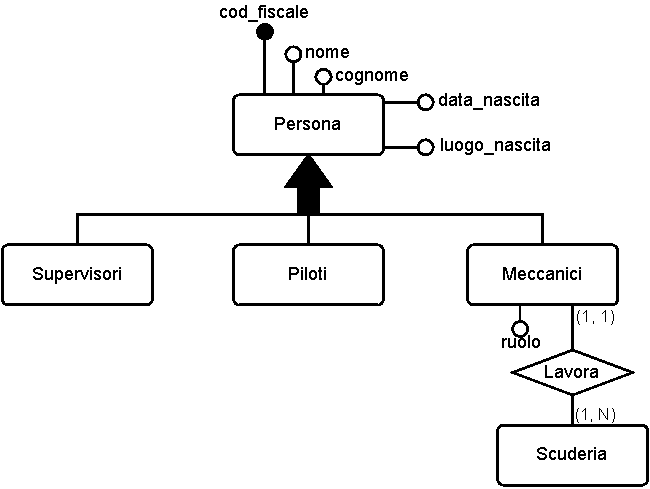
\includegraphics[width=10cm]{../er/gare_persone.pdf}
\end{figure}

\subsubsection{Definizioni delle aziende}
Come aziende, sono state identificate le entità scuderia e sponsor. 
\begin{figure}[H]
    \centering
    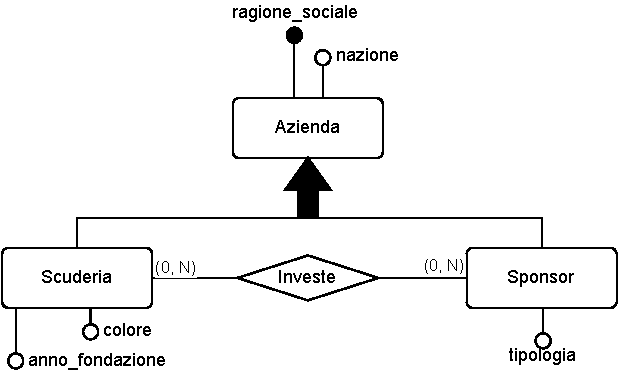
\includegraphics[width=10cm]{../er/gare_aziende.pdf}
\end{figure}

\subsection{Definizioni dei macro-argomenti}
\subsubsection{Definizioni dei partecipanti}
Riguardo i partecipanti, con approccio inside-out, sono state identificate le entità: scuderia, contratto, veicolo, controllo. Oltre a pilota, meccanico, supervisore e sponsor.
\begin{figure}[H]
    \centering
    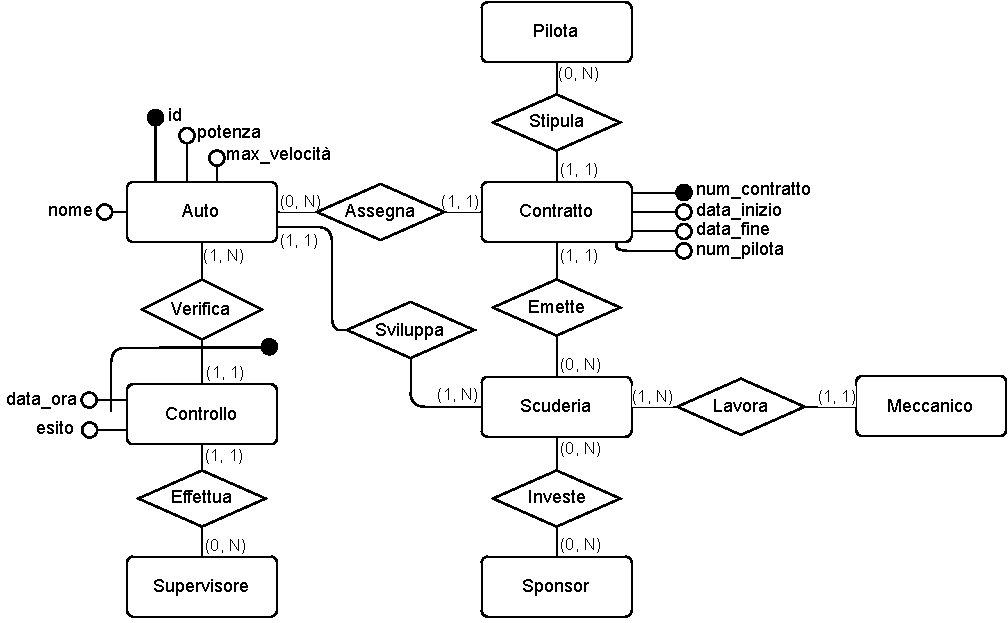
\includegraphics[width=15.5cm]{../er/gare_scuderie.pdf}
\end{figure}

\subsubsection{Definizioni delle competizioni}
Per il concetto di competizione sono state identificate con approccio inside-out le entità: gara, pista, giro, infrazione, pit stop. Oltre a pilota, meccanico e sponsor.
\begin{figure}[H]
    \centering
    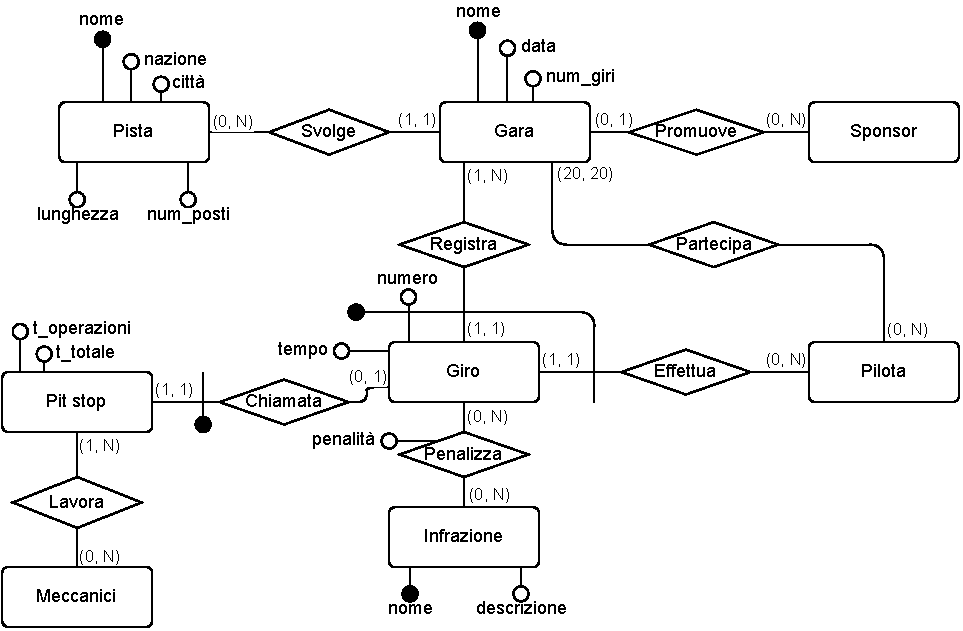
\includegraphics[width=15.5cm]{../er/gare_gara.pdf}
\end{figure}

\newpage
\subsection{Schema finale}
Per chiarezza, nello schema finale, le gerarchie sono state eliminate anticipatamente.
\begin{figure}[H]
    \centering
    \makebox[0cm]{
        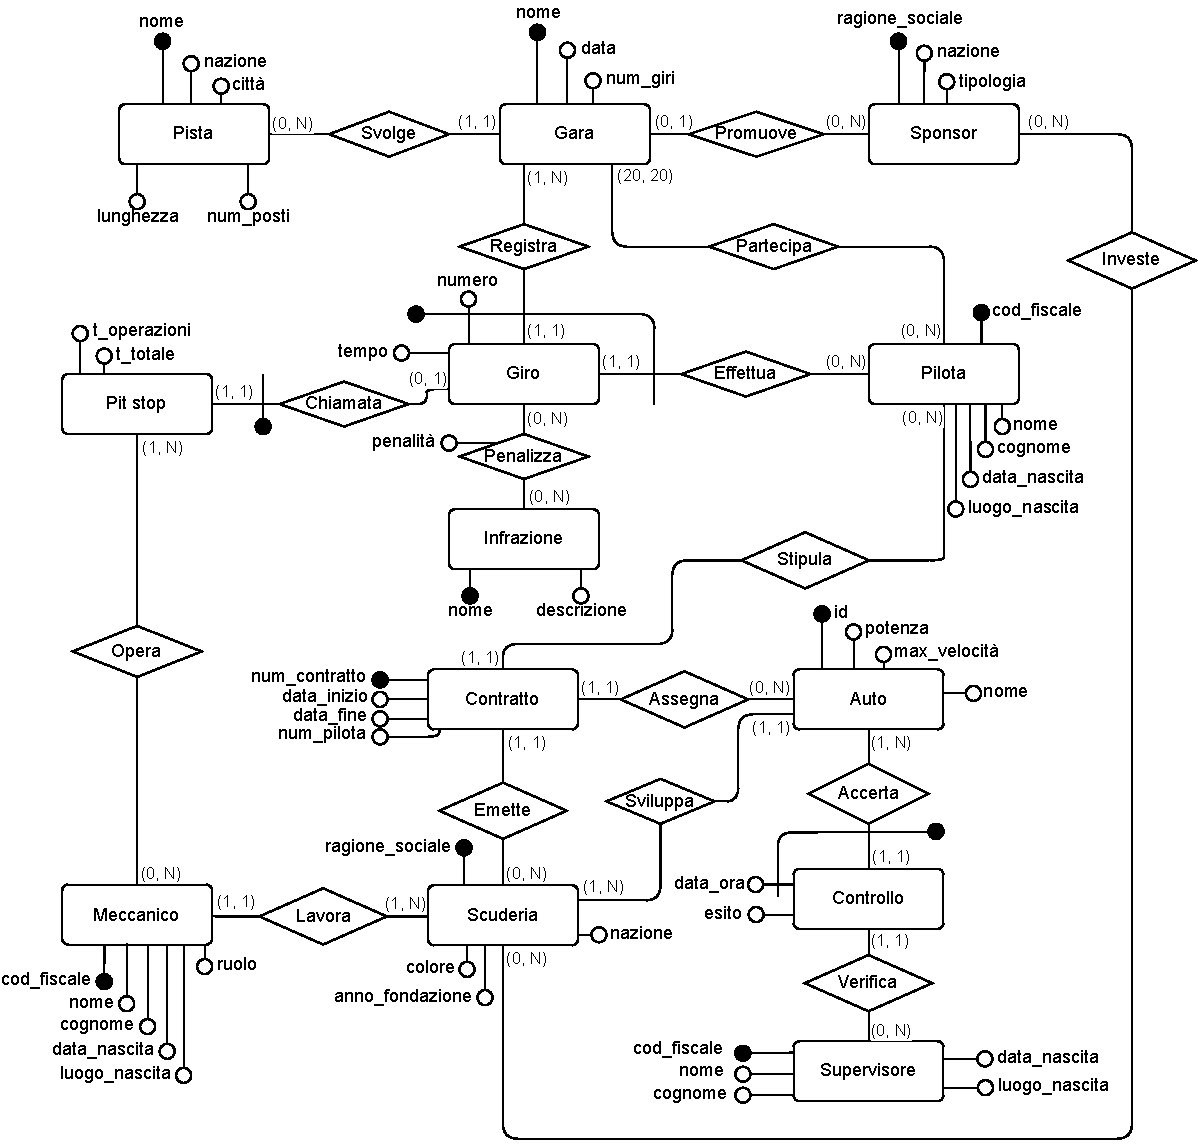
\includegraphics[width=18cm]{../er/gare.pdf}
    }
\end{figure}


\subsection{Dizionario dei dati}

\begin{center}
\makebox[0cm]{
    \begin{tabular}{ |l|p{5.5cm}|p{5cm}|p{4cm}| }
        \hline
        \textbf{Nome entità} & \textbf{Descrizione} & \textbf{Attributi} & \textbf{Identificatore} \\
        
        \hline
        Pilota & 
        Persona che guida un veicolo & 
        \parbox[t]{\linewidth}{Nome (stringa)\\Cognome (stringa)\\Data di nascita (data)\\Luogo di nascita (stringa)} & 
        Codice fiscale (stringa) \\
        
        \hline
        Meccanico &
        Persona che opera su un veicolo & 
        \parbox[t]{\linewidth}{Nome (stringa)\\Cognome (stringa)\\Data di nascita (data)\\Luogo di nascita (stringa)\\Ruolo (stringa)} & 
        Codice fiscale (stringa) \\

        \hline
        Supervisore &
        Persona che effettua dei controlli di regolarità per conto della società organizzante & 
        \parbox[t]{\linewidth}{Nome (stringa)\\Cognome (stringa)\\Data di nascita (data)\\Luogo di nascita (stringa)} & 
        Codice fiscale (stringa) \\

        \hline
        Scuderia &
        Azienda che stipula contratti con piloti e sviluppa auto & 
        \parbox[t]{\linewidth}{Colore (stringa)\\Nazione (stringa)\\Anno di fondazione (numero)} & 
        Ragione sociale (stringa) \\

        \hline
        Sponsor &
        Azienda che investe in gare e/o scuderie & 
        \parbox[t]{\linewidth}{Tipologia (stringa)\\Nazione (stringa)} & 
        Ragione sociale (stringa) \\
        
        \hline
        Contratto &
        Documento stipulato tra un pilota e una scuderia & 
        \parbox[t]{\linewidth}{Data inizio (data)\\Data fine (data)\\Numero pilota (numero)\\Auto assegnata [Veicolo]} & 
        Numero contratto (stringa) \\

        \hline
        Veicolo &
        Autovettura ad elevata velocità di fabbricazione di una scuderia guidata da un pilota &
        \parbox[t]{\linewidth}{Potenza (numero)\\Velocità massima (numero)} & 
        Id (stringa) \\

        \hline
        Controllo &
        Verifica della regolarità di un auto effettuata da un supervisore & 
        \parbox[t]{\linewidth}{Esito (booleano)} & 
        \parbox[t]{\linewidth}{Data e ora (data e ora)\\Id [Veicolo] } \\

        \hline
        Gara &
        Competizione dove 20 piloti gareggiano su una pista per un numero di giri prestabilito & 
        \parbox[t]{\linewidth}{Data e ora (data e ora)\\Numero giri (numero)} & 
        Nome (stringa) \\

        \hline
        Pista &
        Località asfaltata adatta a ospitare gare ad alta velocità & 
        \parbox[t]{\linewidth}{Nazione (stringa)\\Città (stringa)\\Lunghezza (numero)\\Numero posti (numero)} & 
        Nome (stringa) \\

        \hline
        Giro &
        Singola percorrenza completa di pista & 
        \parbox[t]{\linewidth}{Tempo (numero)} & 
        \parbox[t]{\linewidth}{Numero (numero)\\Nome [Gara]\\Codice fiscale [Pilota]} \\ 

        \hline
        Infrazione &
        Evento irregolare durante una gara & 
        \parbox[t]{\linewidth}{Descrizione (stringa)} & 
        Nome (stringa) \\

        \hline
        Pit stop &
        Fase di gara dove l'auto sosta in una specifica area di pista per permettere ai meccanici di effettuare piccole modifiche & 
        \parbox[t]{\linewidth}{Tempo operazioni (numero)\\Tempo totale (numero)} & 
        Chiavi di [Giro] \\

        \hline
    \end{tabular}
}
\end{center}

\begin{center}
    \makebox[0cm]{
        \begin{tabular}{ |l|p{5.5cm}|p{5cm}|p{4cm}| }
            \hline
            \textbf{Nome relazione} & \textbf{Descrizione} & \textbf{Entità coinvolte} & \textbf{Attributi} \\
            
            \hline
            Svolge & 
            Associa la pista su cui si svolge una gara & 
            \parbox[t]{\linewidth}{Pista (0, N)\\Gara (1, 1)} & 
            \parbox[t]{\linewidth}{-} \\

            \hline
            Promuove & 
            Associa l'eventuale sponsor che promuove una gara & 
            \parbox[t]{\linewidth}{Gara (0, 1)\\Sponsor (0, N)} & 
            \parbox[t]{\linewidth}{-} \\

            \hline
            Registra & 
            Associa un giro effettuato in una gara & 
            \parbox[t]{\linewidth}{Gara (1, N)\\Giro (1, 1)} & 
            \parbox[t]{\linewidth}{-} \\

            \hline
            Partecipa & 
            Associa un pilota che partecipa ad una gara & 
            \parbox[t]{\linewidth}{Gara (20, 20)\\Pilota (0, N)} & 
            \parbox[t]{\linewidth}{-} \\

            \hline
            Investe & 
            Associa l'eventuale sponsor che investe in una o più scuderie & 
            \parbox[t]{\linewidth}{Sponsor (0, N)\\Scuderia (0, N)} & 
            \parbox[t]{\linewidth}{-} \\

            \hline
            Chiamata & 
            Associa il giro in cui il pilota viene chiamato per il pit stop & 
            \parbox[t]{\linewidth}{Pit stop (1, 1)\\Giro (0, 1)} & 
            \parbox[t]{\linewidth}{-} \\

            \hline
            Effettua & 
            Associa il giro che viene effettuato dal pilota & 
            \parbox[t]{\linewidth}{Giro (1, 1)\\Pilota (0, N)} & 
            \parbox[t]{\linewidth}{-} \\

            \hline
            Penalizza & 
            Associa la penalità al giro in cui viene commessa l'infrazione & 
            \parbox[t]{\linewidth}{Giro (0, N)\\Penalità (0, N)} & 
            \parbox[t]{\linewidth}{Penalità (numero)} \\

            \hline
            Opera & 
            Associa i meccanici che lavorano durante una sosta al pit stop & 
            \parbox[t]{\linewidth}{Pit stop (1, N)\\Meccanico (0, N)} & 
            \parbox[t]{\linewidth}{-} \\

            \hline
            Stipula & 
            Associa il contratto firmato da un pilota & 
            \parbox[t]{\linewidth}{Pilota (0, N)\\Contratto (1, 1)} & 
            \parbox[t]{\linewidth}{-} \\

            \hline
            Assegna & 
            Associa il veicolo assegnata nel contratto & 
            \parbox[t]{\linewidth}{Contratto (1, 1)\\Veicolo (0, N)} & 
            \parbox[t]{\linewidth}{-} \\

            \hline
            Sviluppa & 
            Associa il veicolo alla scuderia & 
            \parbox[t]{\linewidth}{Veicolo (1, 1)\\Scuderia (1, N)} & 
            \parbox[t]{\linewidth}{-} \\

            \hline
            Emette & 
            Associa la scuderia ai contratti che emette & 
            \parbox[t]{\linewidth}{Contratto (1, 1)\\Scuderia (0, N)} & 
            \parbox[t]{\linewidth}{-} \\

            \hline
            Lavora & 
            Associa un meccanico a una scuderia per la quale lavora & 
            \parbox[t]{\linewidth}{Meccanico (1, 1)\\Scuderia (1, N)} & 
            \parbox[t]{\linewidth}{-} \\

            \hline
            Accerta & 
            Associa un controllo che viene effettuato ad un veicolo & 
            \parbox[t]{\linewidth}{Veicolo (1, N)\\Controllo (1, 1)} & 
            \parbox[t]{\linewidth}{-} \\
            
            \hline
            Verifica & 
            Associa un controllo che viene effettuato da un supervisore & 
            \parbox[t]{\linewidth}{Controllo (1, 1)\\Supervisore (0, N)} & 
            \parbox[t]{\linewidth}{-} \\
            
            \hline
        \end{tabular}
    }
\end{center}

\subsection{Regole aziendali}
\subsubsection{Regole di vincolo}
\begin{enumerate}[label={RV \arabic*}, leftmargin=4em]
    \item Il numero di giri di una gara deve essere $>0$.
    \item Data una gara, il numero di giri effettuato da un pilota, deve essere al più il numero di giri della gara.\\
          Il numero di un giro deve essere quindi compreso tra $[1, \text{numero di giri della gara}]$.
    \item Il numero di posti e la lunghezza di una pista devono essere $>0$. 
    \item Il tempo di un giro deve essere essere $>0$. 
    \item Il tempo delle operazioni e tempo totale dei pit stop devono essere $>0$.
    \item Il tempo della penalità deve essere $>0$.
    \item La potenza e la velocità massima di un veicolo devono essere $>0$.
    \item In un dato istante, un pilota può avere attivo un solo contratto con una scuderia.
    \item La data di inizio di un contratto deve essere antecedente alla data di fine.
    \item I meccanici che operano ad un pit stop devono appartenere alla stessa scuderia del pilota che effettua il giro.
    \item Un contratto deve avere come inizio una data successiva a quella della fondazione della scuderia.
    \item Il veicolo assegnato in un contratto deve appartenere alla scuderia che lo emette.
\end{enumerate}

\subsubsection{Regole di derivazione}
\begin{enumerate}[label={RD \arabic*}, leftmargin=4em]
    \item Il tempo totale impiegato per un giro è dato dalla somma del tempo del giro sommato a quello dell'eventuale pit stop e possibili penalità.
    \item Il vincitore di una gara è il pilota che ha completato il numero di giri previsti nel minor tempo complessivo. In caso di pareggio, si considerano più vincitori.
\end{enumerate}

% \subsubsection{Regole di derivazione}
% \begin{enumerate}[label={RD \arabic*}, leftmargin=4em]
%     \item 
% \end{enumerate}

\section{Progettazione logica}

\subsection{Tavole dei volumi}
\begin{center}
    \begin{tabular}{ |l|l|l| }
        \hline
        \textbf{Concetto} & \textbf{Tipo} & \textbf{Volume} \\
        
        \hline
        Pilota & Entità & 30 \\
        \hline
        Meccanico & Entità & 150 \\
        \hline
        Supervisore & Entità & 15 \\
        \hline
        Scuderia & Entità & 10 \\
        \hline
        Sponsor & Entità & 50 \\
        \hline
        Contratto & Entità & 1400 \\
        \hline
        Veicolo & Entità & 20 \\
        \hline
        Controllo & Entità & 55000 \\ % (73 anni di F1 * 20 piloti per gara * 2 (un controllo a inizio gara e uno alla fine) * 20 gare in media per stagione)
        \hline
        Gara & Entità & 1100 \\
        \hline
        Pista & Entità & 50 \\
        \hline
        Giro & Entità & 70000 \\ % (73 anni di F1 * 20 gare in media per stagione * 50 giri in media per gara)
        \hline
        Infrazione & Entità & 20 \\
        \hline
        Pit stop & Entità & 20000 \\
        \hline
    \end{tabular}
        \quad
    \begin{tabular}{ |l|l|l| }
        \hline
        \textbf{Concetto} & \textbf{Tipo} & \textbf{Volume} \\

        \hline
        Svolge & Relazione & 1100 \\
        \hline
        Promuove & Relazione & 700 \\
        \hline
        Registra & Relazione & 70000 \\
        \hline
        Partecipa & Relazione & 22000 \\
        \hline
        Investe & Relazione & 300 \\
        \hline
        Chiamata & Relazione & 20000 \\
        \hline
        Effettua & Relazione & 70000 \\
        \hline
        Penalizza & Relazione & 8000 \\
        \hline
        Opera & Relazione & 300000 \\ % (volume meccanici 15 * volume pit stop 20000)
        \hline
        Stipula & Relazione & 1400 \\
        \hline
        Assegna & Relazione & 1400 \\
        \hline
        Sviluppa & Relazione & 20 \\
        \hline
        Emette & Relazione & 1400 \\
        \hline
        Lavora & Relazione & 150 \\
        \hline
        Accerta & Relazione & 55000 \\
        \hline
        Verifica & Relazione & 55000 \\
        \hline
    \end{tabular}
\end{center}

\subsection{Tavola delle operazioni}
\begin{center}
    \begin{tabular}{ |l|l| }
        \hline
        \textbf{Operazione} & \textbf{Frequenza} \\

        \hline
        1 & In media 1 volta ogni cinque anni \\
        \hline
        2 & In media 1 volta all'anno \\
        \hline
        3 & $\sim$1000 volte per gara \\
        \hline
        4 & $\sim$20-60 volte per gara \\ 
        \hline
        5 & Poche volte ogni anno \\
        \hline
        6 & In media 2 volte all'anno \\ 
        \hline
        7 & 1 volta all'anno \\
        \hline
        8 & 1 volta per gara \\
        \hline
        9 & 1 volta all'anno \\
        \hline
        10 & 2 volte all'anno \\
        \hline
        11 & 2 volte all'anno \\
        \hline
        12 & 3 volte per gara \\
        \hline
        13 & $\sim$1000 volte per gara \\
        \hline
        14 & 1 volta per gara \\
        \hline
        15 & $\sim$50 volte per gara \\
        \hline
        16 & 1 volta per gara \\
        \hline
        17 & 1 volta per gara \\
        \hline
        18 & 1 volta per gara \\
        \hline
        19 & 1 volta per gara \\
        \hline
        20 & Poche volte all'anno \\
        \hline
        21 & Poche volte all'anno \\
        \hline
    \end{tabular}
\end{center}

\subsection{Ristrutturazione dello schema concettuale}
\subsubsection{Cambio chiave per l'entità Giro}
La chiave dell'entità Giro comprende l'insieme degli attributi numero del giro, nome della gara e id del pilota. Inoltre, l'entità Pit stop utilizza come chiave l'associazione a Giro.\\
Tale approccio rende scomodo lavorare con le due entità, per tale ragione è stato deciso di introdurre un identificatore per l'entità Giro che svolge la funzione di chiave.

\subsubsection{Ristrutturazione relazione Penalizza}
L'associazione Penalizza associa una Infrazione ad un Giro.\\
Poiché ad un Giro possono essere associati più Infrazioni dello stesso tipo, si è ritenuto più chiaro "promuovere" l'associazione Penalizza in una entità definita come segue:

\begin{figure}[H]
    \centering
    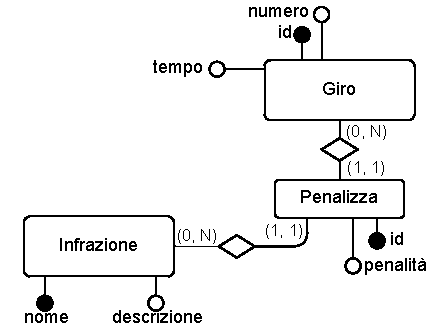
\includegraphics[width=7cm]{../er/penalizza.pdf}
\end{figure}

\subsection{Normalizzazione}

\subsubsection{Associazioni}
Tutte le associazioni dello schema concettuale ristrutturato risultano in forma normale di Boyce e Codd in quanto binarie.

\subsubsection{Entità}
\begin{center}
    \def\arraystretch{1.2}%
    \begin{tabular}{ |p{2cm}|p{14.5cm}| }
        \hline
        \textbf{Entità} & \textbf{Analisi} \\

        \hline
        Pilota & \par{L'unica dipendenza funzionale non banale è tra codice fiscale e il resto degli attributi} \\
        \hline
        Meccanico & \par{L'unica dipendenza funzionale non banale è tra codice fiscale e il resto degli attributi} \\
        \hline
        Supervisore & \par{L'unica dipendenza funzionale non banale è tra codice fiscale e il resto degli attributi} \\
        \hline
        Scuderia & \par{L'unica dipendenza funzionale non banale è tra ragione sociale e il resto degli attributi} \\
        \hline
        Sponsor & \par{L'unica dipendenza funzionale non banale è tra ragione sociale e il resto degli attributi} \\
        \hline
        Contratto & \par{L'unica dipendenza funzionale non banale è tra il numero contratto e il resto degli attributi} \\
        \hline
        Veicolo & \par{L'unica dipendenza funzionale non banale è tra l'id e il resto degli attributi} \\
        \hline
        Controllo & \par{L'unica dipendenza funzionale non banale è \{ data e ora, id dell'auto \} $\rightarrow$ resto degli attributi} \\
        \hline
        Gara & \makecell[l]{
            \parbox[t]{\linewidth}{
                Esiste una dipendenza funzionale non banale tra la pista e il numero dei giri.\\
                È infatti ragionevole assumere che il numero di giri di una gara sia definito in relazione alle caratteristiche della pista.\\
                Si procede quindi a spostare il numero dei giri da Gara a Pista.
            }\\
            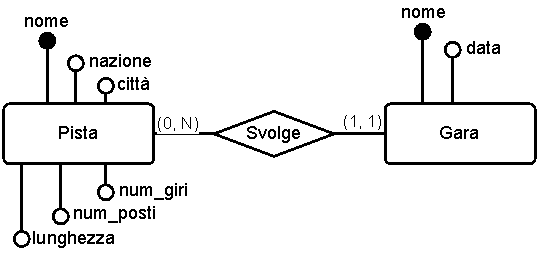
\includegraphics[width=8cm]{../er/norm_pista.pdf}
        } \\
        \hline
        Pista & \par{L'unica dipendenza funzionale non banale è tra il nome della pista e il resto degli attributi} \\
        \hline
        Giro & \par{L'unica dipendenza funzionale non banale è tra l'id del giro e il resto degli attributi} \\
        \hline
        Infrazione & \par{L'unica dipendenza funzionale non banale è tra il nome dell'infrazione e il resto degli attributi} \\
        \hline
        Pit stop & \par{L'unica dipendenza funzionale non banale è tra l'id del giro e il resto degli attributi} \\
        \hline
        Penalizza & \par{L'unica dipendenza funzionale non banale è tra l'id e il resto degli attributi} \\
        \hline
    \end{tabular}
\end{center}
Le entità così definite sono in forma normale di Boyce e Codd.

\subsection{Schema finale ristrutturato}
\begin{figure}[H]
    \centering
    \makebox[0cm]{
        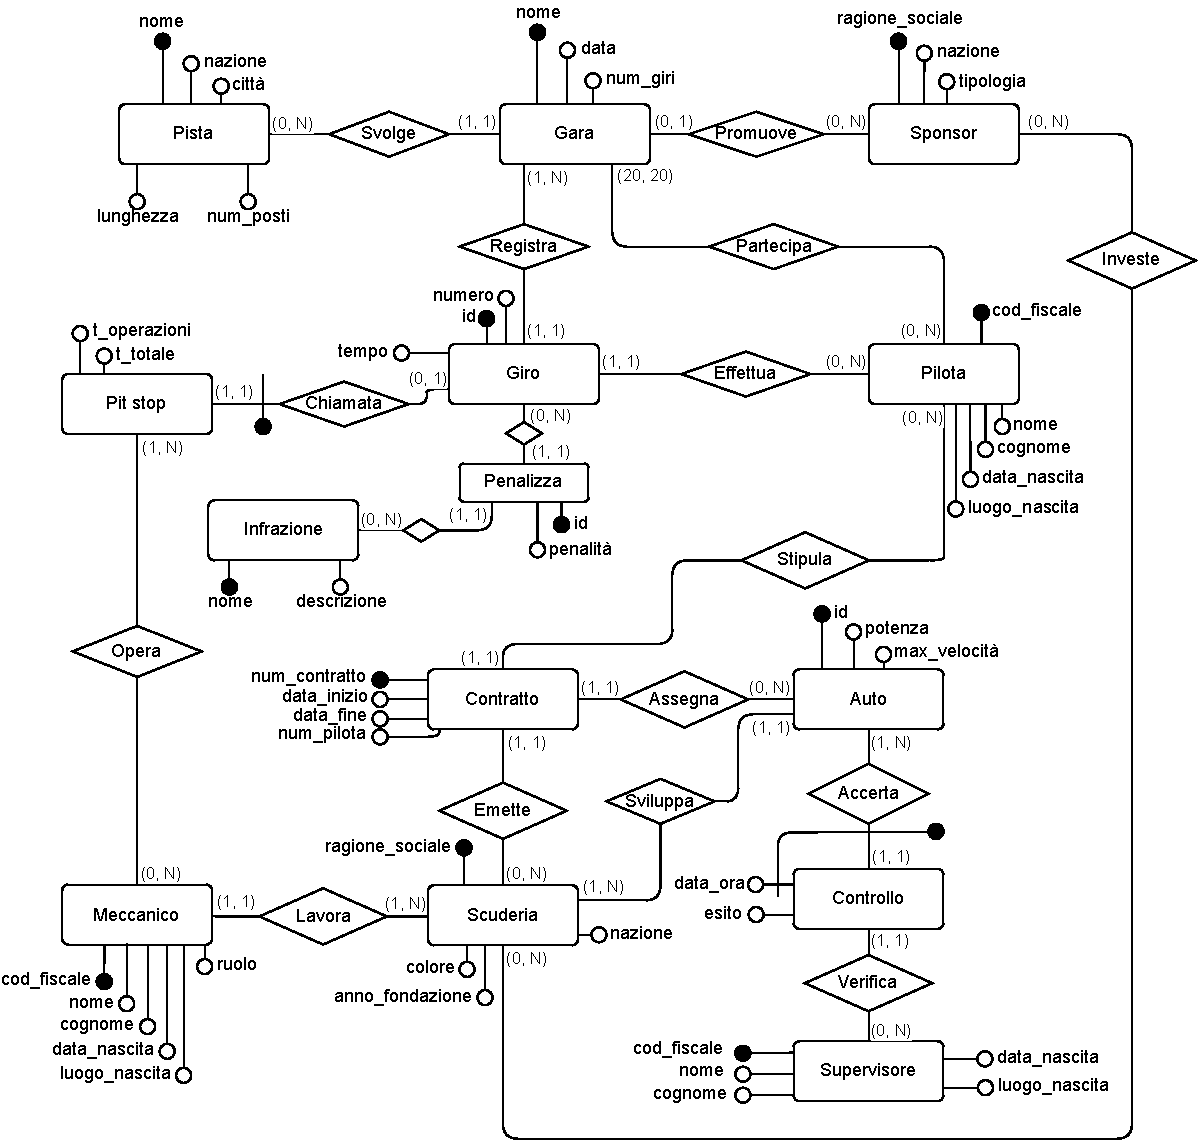
\includegraphics[width=18cm]{../er/finale.pdf}
    }
\end{figure}

\subsection{Traduzione verso il modello relazionale}

\begin{center}
    \makebox[0cm]{
        \def\arraystretch{1.2}%
        \begin{tabular}{ |l|l| }
            \hline
            \textbf{Entità - Relazione} & \textbf{Traduzione} \\

            \hline
            Pilota & Pilota(\underline{codice\_fiscale}, nome, cognome, data\_nascita, luogo\_nascita) \\
            \hline
            Meccanico & \makecell[l]{Meccanico(\underline{codice\_fiscale}, nome, cognome,\\data\_nascita, luogo\_nascita, ruolo, scuderia)} \\
            \hline
            Supervisore & Supervisore(\underline{codice\_fiscale}, nome, cognome, data\_nascita, luogo\_nascita) \\
            \hline
            Scuderia & Scuderia(\underline{ragione\_sociale}, colore, nazione, anno\_fondazione) \\
            \hline
            Sponsor & Sponsor(\underline{ragione\_sociale}, tipologia, nazione) \\
            \hline
            Contratto & Contratto(\underline{numero}, data\_inizio, data\_fine, numero\_pilota, pilota, scuderia, veicolo) \\
            \hline
            Veicolo & Veicolo(\underline{id}, nome, potenza, max\_velocita, scuderia) \\
            \hline
            Controllo & Controllo(\underline{veicolo}, \underline{data\_ora}, esito, supervisore) \\
            \hline
            Gara & Gara(\underline{nome}, data, sponsor, pista) \\
            \hline
            Pista & Pista(\underline{nome}, nazione, citta, lunghezza, num\_posti, num\_giri) \\
            \hline
            Giro & Giro(\underline{id}, numero, tempo, gara, pilota) \\
            \hline
            Infrazione & Infrazione(\underline{nome}, descrizione) \\
            \hline
            Pit stop & Pitstop(\underline{giro}, tempo\_operazione, tempo\_totale) \\
            \hline
            Svolge & Accorpato in Gara \\
            \hline
            Promuove & Accorpato in Gara \\
            \hline
            Registra & Accorpato in Giro \\
            \hline
            Partecipa & Partecipa(\underline{gara}, \underline{pilota}) \\
            \hline
            Investe & Investe(\underline{sponsor}, \underline{scuderia}) \\
            \hline
            Chiamata & Accorpata in Pit Stop \\
            \hline
            Effettua & Accorpata in Giro \\
            \hline
            Penalizza & Penalizza(\underline{id}, giro, infrazione, penalita) \\
            \hline
            Opera & Opera(\underline{pitstop}, \underline{meccanico}) \\
            \hline
            Stipula & Accorpato in Contratto \\
            \hline
            Assegna & Accorpato in Contratto \\
            \hline
            Sviluppa & Accorpato in Veicolo \\
            \hline
            Emette & Accorpato in Contratto \\
            \hline
            Lavora & Accorpato in Meccanico \\
            \hline
            Accerta & Accorpato in Controllo \\
            \hline
            Verifica & Accorpato in Controllo \\
            \hline
        \end{tabular}
    }
\end{center}

\begin{center}
    \makebox[0cm]{
        \def\arraystretch{1.2}%
        \begin{tabular}{ |l|l| }
            \hline
            \textbf{Entità - Relazione} & \textbf{Traduzione} \\

            \hline
            Pilota(\underline{codice\_fiscale}, nome, cognome, data\_nascita, luogo\_nascita) & \makecell[l]{-} \\
            \hline
            \makecell[l]{Meccanico(\underline{codice\_fiscale}, nome, cognome,\\data\_nascita, luogo\_nascita, ruolo, scuderia)} & \makecell[l]{scuderia $\rightarrow$ Scuderia.ragione\_sociale} \\
            \hline
            \makecell[l]{Supervisore(\underline{codice\_fiscale}, nome, cognome,\\data\_nascita, luogo\_nascita)} & \makecell[l]{-} \\
            \hline
            Scuderia(\underline{ragione\_sociale}, colore, nazione, anno\_fondazione) & \makecell[l]{-} \\
            \hline
            Sponsor(\underline{ragione\_sociale}, tipologia, nazione) & \makecell[l]{-} \\
            \hline
            \makecell[l]{Contratto(\underline{numero}, data\_inizio, data\_fine,\\numero\_pilota, pilota, scuderia, veicolo)} & \makecell[l]{pilota $\rightarrow$ Pilota.codice\_fiscale \\ scuderia $\rightarrow$ Scuderia.ragione\_sociale \\ veicolo $\rightarrow$ Veicolo.id} \\
            \hline
            Veicolo(\underline{id}, nome, potenza, max\_velocita, scuderia) & \makecell[l]{scuderia $\rightarrow$ Scuderia.ragione\_sociale} \\ % AGGIORNARE ER -> E' STATO AGGIUNTO IL CAMPO NOME
            \hline
            Controllo(\underline{veicolo}, \underline{data\_ora}, esito, supervisore) & \makecell[l]{veicolo $\rightarrow$ Veicolo.id\\supervisore $\rightarrow$ Supervisore.codice\_fiscale} \\
            \hline
            Gara(\underline{nome}, data\_ora, sponsor, pista) & \makecell[l]{sponsor $\rightarrow$ Sponsor.ragione\_sociale \\ pista $\rightarrow$ Pista.nome} \\
            \hline
            Pista(\underline{nome}, nazione, citta, lunghezza, num\_posti, num\_giri) & \makecell[l]{-} \\
            \hline
            Giro(\underline{id}, numero, tempo, gara, pilota) & \makecell[l]{gara $\rightarrow$ Gara.nome \\ pilota $\rightarrow$ Pilota.codice\_fiscale} \\
            \hline
            Infrazione(\underline{nome}, descrizione) & \makecell[l]{-} \\
            \hline
            Pitstop(\underline{giro}, tempo\_operazione, tempo\_totale) & \makecell[l]{giro $\rightarrow$ Giro.id} \\
            \hline
            Partecipa(\underline{gara}, \underline{pilota}) & \makecell[l]{gara $\rightarrow$ Gara.nome \\ pilota $\rightarrow$ Pilota.codice\_fiscale} \\
            \hline
            Investe(\underline{sponsor}, \underline{scuderia}) & \makecell[l]{sponsor $\rightarrow$ Sponsor.ragione\_sociale \\ scuderia $\rightarrow$ Scuderia.ragione\_sociale } \\
            \hline
            Penalizza(\underline{id}, giro, infrazione, penalita) & \makecell[l]{giro $\rightarrow$ Giro.id \\ infrazione $\rightarrow$ Infrazione.nome} \\
            \hline
            Opera(\underline{pitstop}, \underline{meccanico}) & \makecell[l]{pitstop $\rightarrow$ Pitstop.giro \\ meccanico $\rightarrow$ Meccanico.codice\_fiscale} \\
            \hline
        \end{tabular}
    }
\end{center}



\section{Codifica SQL}

\subsection{Definizione dello schema}

\begin{lstlisting}[ language=SQL ]
CREATE TABLE Pilota(
    codice_fiscale CHAR(20) PRIMARY KEY,
    nome VARCHAR(100) NOT NULL,
    cognome VARCHAR(100) NOT NULL,
    data_nascita DATE NOT NULL,
    luogo_nascita VARCHAR(100) NOT NULL
);
\end{lstlisting}

\begin{lstlisting}[ language=SQL ]
CREATE TABLE Meccanico(
    codice_fiscale CHAR(20) PRIMARY KEY,
    nome VARCHAR(100) NOT NULL,
    cognome VARCHAR(100) NOT NULL,
    data_nascita DATE NOT NULL,
    luogo_nascita VARCHAR(100) NOT NULL,
    ruolo VARCHAR(100) NOT NULL,
    scuderia VARCHAR(100) NOT NULL REFERENCES Scuderia(ragione_sociale) 
                                   ON DELETE CASCADE ON UPDATE CASCADE
);
\end{lstlisting}

\begin{lstlisting}[ language=SQL ]
CREATE TABLE Supervisore(
    codice_fiscale CHAR(20) PRIMARY KEY,
    nome VARCHAR(100) NOT NULL,
    cognome VARCHAR(100) NOT NULL,
    data_nascita DATE NOT NULL,
    luogo_nascita VARCHAR(100) NOT NULL
);
\end{lstlisting}

\begin{lstlisting}[ language=SQL ]
CREATE TABLE Scuderia(
    ragione_sociale VARCHAR(100) PRIMARY KEY,
    colore VARCHAR(100) NOT NULL,
    nazione VARCHAR(100) NOT NULL,
    anno_fondazione SMALLINT NOT NULL,
    CHECK (anno_fondazione > 0)
);
\end{lstlisting}

\begin{lstlisting}[ language=SQL ]
CREATE TABLE Sponsor(
    ragione_sociale VARCHAR(100) PRIMARY KEY,
    tipologia VARCHAR(100) NOT NULL,
    nazione VARCHAR(100) NOT NULL
);
\end{lstlisting}

\begin{lstlisting}[ language=SQL ]
CREATE TABLE Contratto(
    numero INTEGER PRIMARY KEY AUTOINCREMENT,
    data_inizio DATETIME NOT NULL,
    data_fine DATETIME NOT NULL,
    numero_pilota TINYINT NOT NULL,
    pilota VARCHAR(100) REFERENCES Pilota(codice_fiscale) 
                        ON DELETE RESTRICT ON UPDATE CASCADE,
    scuderia VARCHAR(100) REFERENCES Scuderia(ragione_sociale) 
                          ON DELETE RESTRICT ON UPDATE CASCADE,
    veicolo INTEGER REFERENCES Veicolo(id) 
                    ON DELETE RESTRICT ON UPDATE CASCADE,
    CHECK (data_fine > data_inizio AND numero_pilota > 0)
);
\end{lstlisting}

\begin{lstlisting}[ language=SQL ]
CREATE TABLE Veicolo(
    id INTEGER PRIMARY KEY AUTOINCREMENT,
    nome VARCHAR(100) NOT NULL,
    potenza INTEGER NOT NULL,
    max_velocita INTEGER NOT NULL,
    scuderia VARCHAR(100) REFERENCES Scuderia(ragione_sociale) 
                          ON DELETE CASCADE ON UPDATE CASCADE,
    CHECK (potenza > 0 AND max_velocita > 0)
);
\end{lstlisting}

\begin{lstlisting}[ language=SQL ]
CREATE TABLE Controllo(
    veicolo INTEGER REFERENCES Veicolo(id),
    data_ora DATETIME,
    esito BOOLEAN NOT NULL,
    supervisore VARCHAR(100) REFERENCES Supervisore(codice_fiscale) 
                             ON DELETE SET NULL ON UPDATE CASCADE,
    PRIMARY KEY (veicolo, data_ora)
);
\end{lstlisting}

\newpage
\begin{lstlisting}[ language=SQL ]
CREATE TABLE Gara(
    nome VARCHAR(100) PRIMARY KEY,
    data_ora DATETIME NOT NULL,
    sponsor VARCHAR(100) REFERENCES Sponsor(ragione_sociale) 
                         ON DELETE RESTRICT ON UPDATE CASCADE,
    pista VARCHAR(100) REFERENCES Pista(nome) 
                       ON DELETE RESTRICT ON UPDATE CASCADE
);
\end{lstlisting}

\begin{lstlisting}[ language=SQL ]
CREATE TABLE Pista(
    nome VARCHAR(100) PRIMARY KEY,
    nazione VARCHAR(100) NOT NULL,
    citta VARCHAR(100) NOT NULL,
    lunghezza INTEGER NOT NULL,
    num_posti INTEGER NOT NULL,
    num_giri TINYINT NOT NULL,
    CHECK (lunghezza > 0 AND num_posti >= 0 AND num_giri > 0)
);
\end{lstlisting}

\begin{lstlisting}[ language=SQL ]
CREATE TABLE Giro(
    id INTEGER PRIMARY KEY AUTOINCREMENT,
    numero INTEGER NOT NULL,
    tempo INTEGER NOT NULL,
    gara VARCHAR(100) REFERENCES Gara(nome) 
                      ON DELETE RESTRICT ON UPDATE CASCADE,
    pilota VARCHAR(100) REFERENCES Pilota(codice_fiscale) 
                        ON DELETE RESTRICT ON UPDATE CASCADE,
    CHECK (numero > 0 AND tempo > 0)
);
\end{lstlisting}

\begin{lstlisting}[ language=SQL ]
CREATE TABLE Infrazione(
    nome VARCHAR(100) PRIMARY KEY,
    descrizione VARCHAR(500) NOT NULL
);
\end{lstlisting}

\begin{lstlisting}[ language=SQL ]
CREATE TABLE Pitstop(
    giro INTEGER PRIMARY KEY REFERENCES Giro(id) 
                             ON DELETE CASCADE ON UPDATE CASCADE,
    tempo_operazione INTEGER NOT NULL,
    tempo_totale INTEGER NOT NULL,
    CHECK (tempo_operazione > 0 AND tempo_totale > tempo_operazione)
);
\end{lstlisting}

\begin{lstlisting}[ language=SQL ]
CREATE TABLE Partecipa(
    gara VARCHAR(100) REFERENCES Gara(nome) 
                      ON DELETE CASCADE ON UPDATE CASCADE,
    pilota VARCHAR(100) REFERENCES Pilota(codice_fiscale) 
                        ON DELETE RESTRICT ON UPDATE CASCADE,
    PRIMARY KEY (gara, pilota)
);
\end{lstlisting}

\begin{lstlisting}[ language=SQL ]
CREATE TABLE Investe(
    sponsor VARCHAR(100) REFERENCES Sponsor(ragione_sociale) 
                         ON DELETE CASCADE ON UPDATE CASCADE,
    scuderia VARCHAR(100) REFERENCES Scuderia(ragione_sociale) 
                          ON DELETE CASCADE ON UPDATE CASCADE,
    PRIMARY KEY (sponsor, scuderia)
);
\end{lstlisting}

\newpage
\begin{lstlisting}[ language=SQL ]
CREATE TABLE Penalizza(
    id INTEGER PRIMARY KEY AUTOINCREMENT,
    giro INTEGER REFERENCES Giro(id) 
                 ON DELETE CASCADE ON UPDATE CASCADE,
    infrazione VARCHAR(100) REFERENCES Infrazione(nome) 
                            ON DELETE RESTRICT ON UPDATE CASCADE,
    penalita INTEGER NOT NULL,
    CHECK (penalita > 0)
);
\end{lstlisting}

\begin{lstlisting}[ language=SQL ]
CREATE TABLE Opera(
    pitstop INTEGER REFERENCES Pitstop(giro) 
                    ON DELETE CASCADE ON UPDATE CASCADE,
    meccanico VARCHAR(100) REFERENCES Meccanico(codice_fiscale) 
                           ON DELETE RESTRICT ON UPDATE CASCADE,
    PRIMARY KEY (pitstop, meccanico)
);
\end{lstlisting}



\subsection{Codifica delle operazioni}

\subsubsection{Operazione 1}
Inserire una nuova scuderia.
\begin{lstlisting}[ language=SQL ]
INSERT INTO Scuderia (ragione_sociale, colore, nazione, anno_fondazione) VALUES
    ('<ragione sociale>', '<colore>', '<nazione>', <anno fondazione>);
\end{lstlisting}


\subsubsection{Operazione 2}
Inserire una nuova gara.
\begin{lstlisting}[ language=SQL ]
INSERT INTO Gara (nome, data_ora, sponsor, pista) VALUES 
    ('<nome>', '<data e ora>', <sponsor o NULL>, '<nome pista>');
\end{lstlisting}


\subsubsection{Operazione 3}
Inserire il tempo di un giro del pilota sulla pista.
\begin{lstlisting}[ language=SQL ]
INSERT INTO Giro (id, numero, tempo, gara, pilota) VALUES 
    (NULL, <numero>, <tempo>, '<nome gara>', '<codice fiscale pilota>');
\end{lstlisting}


\subsubsection{Operazione 4}
Inserire il tempo pit stop.
\begin{lstlisting}[ language=SQL ]
INSERT INTO Pitstop (giro, tempo_operazione, tempo_totale) VALUES 
    (<id giro>, <tempo operazione>, <tempo totale>);
\end{lstlisting}


\subsubsection{Operazione 5}
Inserire un nuovo contratto tra pilota e scuderia.
\begin{lstlisting}[ language=SQL ]
INSERT INTO Contratto 
    (numero, data_inizio, data_fine, numero_pilota, pilota, scuderia, veicolo) 
VALUES 
    (NULL, '<data inizio>', '<data fine>', <numero pilota>, 
    '<codice fiscale pilota>', '<ragione sociale scuderia>', <id veicolo>);
\end{lstlisting}


\subsubsection{Operazione 6}
Incrementare la potenza e la velocità massima dei veicoli di una data scuderia.
\begin{lstlisting}[ language=SQL ]
UPDATE Veicolo
SET potenza = potenza + 50,
    max_velocita = max_velocita + 5
WHERE Veicolo.scuderia = '<Ragione sociale scuderia>';   
\end{lstlisting}


\subsubsection{Operazione 7}
Visualizzare la lunghezza media, massima e minima delle piste.
\begin{lstlisting}[ language=SQL ]
SELECT AVG(lunghezza) AS Media, MAX(lunghezza) AS Massimo, MIN(lunghezza) AS Minimo
FROM Pista;
\end{lstlisting}

\begin{table}[H]
    \centering
    \begin{tabular}{|l|l|l|}
    \hline
        \textbf{Media} & \textbf{Massimo} & \textbf{Minimo} \\ \hline
        5151.181818181818 & 7004 & 3337 \\ \hline
    \end{tabular}
\end{table}


\subsubsection{Operazione 8}
Visualizzare lo sponsor di una gara.
\begin{lstlisting}[ language=SQL ]
SELECT S.*
FROM Gara AS G INNER JOIN Sponsor AS S ON G.sponsor = S.ragione_sociale
WHERE G.nome = '<Nome gara>';
\end{lstlisting}

\begin{table}[H]
    \centering
    \begin{tabular}{|l|l|l|}
    \hline
        \textbf{ragione\_sociale} & \textbf{tipologia} & \textbf{nazione} \\ \hline
        Rolex & Orologeria & Svizzera \\ \hline
    \end{tabular}
\end{table}


\subsubsection{Operazione 9}
Visualizzare lo sponsor più presente.
\begin{lstlisting}[ language=SQL ]
SELECT sponsor.ragione_sociale, COUNT(*) AS num_comparse
FROM (SELECT Investe.sponsor AS ragione_sociale FROM Investe 
      UNION ALL 
      SELECT Gara.sponsor AS ragione_sociale FROM Gara) AS sponsor
GROUP BY sponsor.ragione_sociale
HAVING num_comparse = (
    SELECT COUNT(*) AS comparse
    FROM (
        SELECT Investe.sponsor AS ragione_sociale FROM Investe 
        UNION ALL 
        SELECT Gara.sponsor AS ragione_sociale FROM Gara
    ) AS sponsor
    GROUP BY sponsor.ragione_sociale
    ORDER BY comparse DESC LIMIT 1
);
\end{lstlisting}

\begin{table}[H]
    \centering
    \begin{tabular}{|l|l|}
    \hline
        \textbf{ragione\_sociale} & \textbf{num\_comparse} \\ \hline
        Acer & 6 \\ \hline
        Coca Cola & 6 \\ \hline
        Nike & 6 \\ \hline
    \end{tabular}
\end{table}


\subsubsection{Operazione 10}
Visualizzare la scuderia con cui un pilota ha un contratto in una determinata data.
\begin{lstlisting}[ language=SQL ]
SELECT C.scuderia
FROM Contratto AS C
WHERE ('<Data>' BETWEEN C.data_inizio AND C.data_fine) AND
      C.pilota = '<Codice fiscale pilota>';
\end{lstlisting}

\begin{table}[H]
    \centering
    \begin{tabular}{|l|}
    \hline
        \textbf{scuderia} \\ \hline
        Red Bull \\ \hline
    \end{tabular}
\end{table}


\subsubsection{Operazione 11}
Visualizzare nome, cognome e numero di gara dei piloti di una data scuderia con contratto attivo al momento attuale.
\begin{lstlisting}[ language=SQL ]
SELECT P.cognome, P.nome, C.numero_pilota
FROM Contratto AS C INNER JOIN Scuderia AS S ON C.scuderia = S.ragione_sociale 
                    INNER JOIN Pilota AS P ON P.codice_fiscale = C.pilota
WHERE S.ragione_sociale = '<Ragione sociale scuderia>' AND
      (date('now') BETWEEN C.data_inizio AND C.data_fine);
\end{lstlisting}

\begin{table}[H]
    \centering
    \begin{tabular}{|l|l|l|}
    \hline
        \textbf{cognome} & \textbf{nome} & \textbf{numero\_pilota} \\ \hline
        Leclerc & Charles & 16 \\ \hline
        Sainz & Carlos & 55 \\ \hline
    \end{tabular}
\end{table}


\subsubsection{Operazione 12}
Visualizzare i piloti e la scuderia con cui gareggiano per una data gara raggruppandoli per scuderia.
\begin{lstlisting}[ language=SQL ]
SELECT D.nome, D.cognome, C.scuderia
FROM Partecipa AS P INNER JOIN Pilota AS D ON P.pilota = D.codice_fiscale
                    INNER JOIN Contratto AS C ON D.codice_fiscale = C.pilota
                    INNER JOIN Gara AS G ON P.gara = G.nome
WHERE P.gara = '<Nome gara>' AND
      (G.data_ora BETWEEN C.data_inizio AND C.data_fine)
ORDER BY C.scuderia;
\end{lstlisting}

\begin{table}[H]
    \centering
    \begin{tabular}{|l|l|l|}
    \hline
        \textbf{nome} & \textbf{cognome} & \textbf{scuderia} \\ \hline
        Valtteri & Bottas & Alfa Romeo \\ \hline
        Zhou & Guanyu & Alfa Romeo \\ \hline
        Pierre & Gasly & AlphaTauri \\ \hline
        Yuki & Tsunoda & AlphaTauri \\ \hline
        Fernando & Alonso & Alpine \\ \hline
        Esteban & Ocon & Alpine \\ \hline
        Lance & Stroll & Aston Martin \\ \hline
        Sebastian & Vettel & Aston Martin \\ \hline
        Charles & Leclerc & Ferrari \\ \hline
        Carlos & Sainz & Ferrari \\ \hline
        Kevin & Magnussen & Haas \\ \hline
        Mick & Schumacher & Haas \\ \hline
        Daniel & Ricciardo & McLaren \\ \hline
        Lando & Norris & McLaren \\ \hline
        George & Russell & Mercedes \\ \hline
        Lewis & Hamilton & Mercedes \\ \hline
        Max & Verstappen & Red Bull \\ \hline
        Sergio & Pérez & Red Bull \\ \hline
        Alexander & Albon & Williams \\ \hline
        Nicholas & Latifi & Williams \\ \hline
    \end{tabular}
\end{table}


\subsubsection{Operazione 13}
Visualizzare il tempo reale di un giro.
\begin{lstlisting}[ language=SQL ]
CREATE VIEW IF NOT EXISTS GiroReale AS
SELECT Giro.id, Giro.pilota, Giro.gara, Giro.numero, 
       (
         Giro.tempo + 
         COALESCE(SUM(Penalizza.penalita), 0) + 
         COALESCE(Pitstop.tempo_totale, 0)
       ) AS tempo_totale
FROM Giro LEFT OUTER JOIN Penalizza ON Giro.id = Penalizza.giro
          LEFT OUTER JOIN Pitstop ON Giro.id = Pitstop.giro
GROUP BY Giro.id, Giro.pilota, Giro.gara, Giro.numero;

SELECT * FROM GiroReale;
\end{lstlisting}

\begin{center}
    \begin{table}[H]
        \centering
        \begin{tabular}{|l|l|l|l|l|}
            \hline
            \textbf{id} & \textbf{pilota} & \textbf{gara} & \textbf{numero} & \textbf{tempo\_totale} \\ \hline
            0 & RSSGRG98B15Z114G & Bahrain Grand Prix & 1 & 179548 \\ \hline
            1 & RSSGRG98B15Z114G & Bahrain Grand Prix & 2 & 63654 \\ \hline
            2 & RSSGRG98B15Z114G & Bahrain Grand Prix & 3 & 125114 \\ \hline
        \end{tabular}
    \end{table}
    \vspace*{-1em}
    \dots
\end{center}


\newpage
\subsubsection{Operazione 14}
Visualizzare il pilota con il tempo migliore su una data pista.
\begin{lstlisting}[ language=SQL ]
SELECT Pilota.nome, Pilota.cognome, GiroReale.tempo_totale
FROM GiroReale INNER JOIN Gara ON GiroReale.gara = Gara.nome
               INNER JOIN Pilota ON GiroReale.pilota = Pilota.codice_fiscale
WHERE Gara.pista = '<Nome pista>' AND
      GiroReale.tempo_totale = (
         SELECT MIN(GiroReale.tempo_totale)
         FROM GiroReale INNER JOIN Gara ON GiroReale.gara = Gara.nome
         WHERE Gara.pista = '<Nome pista>'
      );
\end{lstlisting}

\begin{table}[H]
    \centering
    \begin{tabular}{|l|l|l|}
    \hline
        \textbf{nome} & \textbf{cognome} & \textbf{tempo\_totale} \\ \hline
        George & Russell & 61749 \\ \hline
    \end{tabular}
\end{table}


\subsubsection{Operazione 15}
Visualizzare la classifica (finale o temporanea) di una data gara.
\begin{lstlisting}[ language=SQL ]
SELECT Pilota.nome, Pilota.cognome, Contratto.scuderia, COUNT(GiroReale.id) AS num_giri, 
       SUM(GiroReale.tempo_totale) AS tempo_gara
FROM GiroReale INNER JOIN Pilota ON GiroReale.pilota = Pilota.codice_fiscale
               INNER JOIN Contratto ON Pilota.codice_fiscale = Contratto.pilota
               INNER JOIN Gara ON GiroReale.gara = Gara.nome
WHERE GiroReale.gara = '<Nome gara>' AND
      (Gara.data_ora BETWEEN Contratto.data_inizio AND Contratto.data_fine)
GROUP BY GiroReale.pilota, Pilota.nome, Pilota.cognome, Contratto.scuderia
ORDER BY num_giri DESC, tempo_gara ASC;
\end{lstlisting}

\begin{table}[H]
    \centering
    \begin{tabular}{|l|l|l|l|l|}
    \hline
        \textbf{nome} & \textbf{cognome} & \textbf{scuderia} & \textbf{num\_giri} & \textbf{tempo\_gara} \\ \hline
        Lewis & Hamilton & Mercedes & 5 & 457808 \\ \hline
        Alexander & Albon & Williams & 5 & 466535 \\ \hline
        Pierre & Gasly & AlphaTauri & 5 & 474886 \\ \hline
        George & Russell & Mercedes & 5 & 475413 \\ \hline
        Sebastian & Vettel & Aston Martin & 5 & 476566 \\ \hline
        Charles & Leclerc & Ferrari & 5 & 528565 \\ \hline
        Zhou & Guanyu & Alfa Romeo & 5 & 536496 \\ \hline
        Mick & Schumacher & Haas & 5 & 542647 \\ \hline
        Daniel & Ricciardo & McLaren & 5 & 554410 \\ \hline
        Yuki & Tsunoda & AlphaTauri & 5 & 567581 \\ \hline
        Nicholas & Latifi & Williams & 4 & 371216 \\ \hline
        Max & Verstappen & Red Bull & 4 & 505714 \\ \hline
        Sergio & Pérez & Red Bull & 3 & 324935 \\ \hline
        Fernando & Alonso & Alpine & 3 & 349770 \\ \hline
        Lance & Stroll & Aston Martin & 2 & 210603 \\ \hline
        Esteban & Ocon & Alpine & 1 & 98857 \\ \hline
        Kevin & Magnussen & Haas & 1 & 105440 \\ \hline
        Carlos & Sainz & Ferrari & 1 & 107001 \\ \hline
        Valtteri & Bottas & Alfa Romeo & 1 & 115063 \\ \hline
        Lando & Norris & McLaren & 1 & 134215 \\ \hline
    \end{tabular}
\end{table}


\subsubsection{Operazione 16}
Visualizzare i vincitori di una gara.
\begin{lstlisting}[ language=SQL ]
SELECT Pilota.nome, Pilota.cognome, Contratto.scuderia
FROM GiroReale INNER JOIN Pilota ON GiroReale.pilota = Pilota.codice_fiscale
               INNER JOIN Contratto ON Pilota.codice_fiscale = Contratto.pilota
               INNER JOIN Gara ON GiroReale.gara = Gara.nome
               INNER JOIN Pista ON Gara.pista = Pista.nome
WHERE GiroReale.gara = '<Nome gara>' AND
      (Gara.data_ora BETWEEN Contratto.data_inizio AND Contratto.data_fine)
GROUP BY GiroReale.pilota, Pilota.nome, Pilota.cognome, Contratto.scuderia
HAVING SUM(GiroReale.tempo_totale) = (
            SELECT SUM(GiroReale.tempo_totale) AS tempo_gara
            FROM GiroReale
            WHERE GiroReale.gara = '<Nome gara>'
            GROUP BY GiroReale.pilota
            ORDER BY COUNT(GiroReale.id) DESC, tempo_gara ASC LIMIT 1
       ) AND
       COUNT(GiroReale.id) = Pista.num_giri
ORDER BY COUNT(GiroReale.id) DESC, SUM(GiroReale.tempo_totale) ASC;
\end{lstlisting}

\begin{table}[H]
    \centering
    \begin{tabular}{|l|l|l|}
    \hline
        \textbf{nome} & \textbf{cognome} & \textbf{scuderia} \\ \hline
        Lewis & Hamilton & Mercedes \\ \hline
    \end{tabular}
\end{table}


\subsubsection{Operazione 17}
Visualizzare in ordine decrescente i piloti e il loro numero di vittorie.
\begin{lstlisting}[ language=SQL ]
CREATE VIEW IF NOT EXISTS Vincitore AS
SELECT Pilota.nome, Pilota.cognome, Pilota.codice_fiscale, 
       COUNT(vincitori.gara) AS vittorie
FROM Pilota LEFT OUTER JOIN (
        SELECT GiroReale.pilota, GiroReale.gara
        FROM GiroReale INNER JOIN Gara ON GiroReale.gara = Gara.nome
                       INNER JOIN Pista ON Gara.pista = Pista.nome
        GROUP BY GiroReale.gara, GiroReale.pilota
        HAVING SUM(GiroReale.tempo_totale) = (
                    SELECT SUM(GR.tempo_totale)
                    FROM GiroReale AS GR
                    WHERE GR.gara = GiroReale.gara
                    GROUP BY GR.pilota
                    ORDER BY COUNT(GR.id) DESC, SUM(GR.tempo_totale) ASC LIMIT 1
                ) AND
                COUNT(GiroReale.id) = Pista.num_giri
     ) AS vincitori ON Pilota.codice_fiscale = vincitori.pilota
GROUP BY Pilota.codice_fiscale
ORDER BY vittorie DESC;

SELECT * FROM Vincitore;
\end{lstlisting}

\begin{table}[H]
    \centering
    \begin{tabular}{|l|l|l|l|}
    \hline
        \textbf{nome} & \textbf{cognome} & \textbf{codice\_fiscale} & \textbf{vittorie} \\ \hline
        Lewis & Hamilton & HMLLWS85A07Z114F & 4 \\ \hline
        Charles & Leclerc & LCLCRL97R16Z123N & 4 \\ \hline
        Kevin & Magnussen & MGNKVN92R05Z107H & 3 \\ \hline
        Valtteri & Bottas & BTTVTT89M28Z109S & 2 \\ \hline
        Sergio & Pérez & PRZSRG90A26Z514G & 2 \\ \hline
        George & Russell & RSSGRG98B15Z114G & 2 \\ \hline
        Alexander & Albon & LBNLND96C23Z241E & 1 \\ \hline
        Daniel & Ricciardo & RCCDNL89L01Z700U & 1 \\ \hline
        Mick & Schumacher & SCHMCK99C22Z110X & 1 \\ \hline
        Carlos & Sainz & SNZCLS94P01Z131Y & 1 \\ \hline
        Max & Verstappen & VRSMXA97P30Z126X & 1 \\ \hline
        Esteban & Ocon & CNOSBN96P17Z110F & 0 \\ \hline
        Pierre & Gasly & GSLPRR96B07Z110S & 0 \\ \hline
        Fernando & Alonso & LNSFNN81L29Z131M & 0 \\ \hline
        Nicholas & Latifi & LTFNHL95H29Z401V & 0 \\ \hline
        Lando & Norris & NRRLND99S13Z114I & 0 \\ \hline
        Lance & Stroll & STRLNC98R29Z401K & 0 \\ \hline
        Yuki & Tsunoda & TSNYKU00E11Z219F & 0 \\ \hline
        Sebastian & Vettel & VTTSST87L03Z110A & 0 \\ \hline
        Zhou & Guanyu & ZHOGNY99E30Z210K & 0 \\ \hline
    \end{tabular}
\end{table}


\subsubsection{Operazione 18}
Visualizzare il pilota più giovane ad aver vinto almeno una gara.
\begin{lstlisting}[ language=SQL ]
SELECT Pilota.nome, Pilota.cognome, Pilota.data_nascita
FROM Vincitore INNER JOIN Pilota ON Vincitore.codice_fiscale = Pilota.codice_fiscale
WHERE Vincitore.vittorie > 0 AND
   Pilota.data_nascita = (
    SELECT MAX(Pilota.data_nascita)
    FROM Vincitore INNER JOIN Pilota ON Vincitore.codice_fiscale = Pilota.codice_fiscale
    WHERE Vincitore.vittorie > 0
   );
\end{lstlisting}

\begin{table}[H]
    \centering
    \begin{tabular}{|l|l|l|}
    \hline
        \textbf{nome} & \textbf{cognome} & \textbf{data\_nascita} \\ \hline
        Mick & Schumacher & 1999-03-22 \\ \hline
    \end{tabular}
\end{table}


\subsubsection{Operazione 19}
Visualizzare pilota e scuderia con il pitstop più veloce.
\begin{lstlisting}[ language=SQL ]
SELECT Pilota.nome, Pilota.cognome, Contratto.scuderia, Pitstop.tempo_operazione, 
       Gara.nome AS nome_gara
FROM Pitstop INNER JOIN Giro ON Pitstop.giro = Giro.id
             INNER JOIN Pilota ON Giro.pilota = Pilota.codice_fiscale
             INNER JOIN Gara ON Giro.gara = Gara.nome
             INNER JOIN Contratto ON Pilota.codice_fiscale = Contratto.pilota
WHERE (Gara.data_ora BETWEEN Contratto.data_inizio AND Contratto.data_fine) AND
      Pitstop.tempo_operazione = (SELECT MIN(Pitstop.tempo_operazione)
                                  FROM Pitstop);
\end{lstlisting}

\begin{table}[H]
    \centering
    \begin{tabular}{|l|l|l|l|l|}
    \hline
        \textbf{nome} & \textbf{cognome} & \textbf{scuderia} & \textbf{tempo\_operazione} & \textbf{nome\_gara} \\ \hline
        Kevin & Magnussen & Haas & 1014 & Grande Prêmio de São Paulo \\ \hline
    \end{tabular}
\end{table}


\subsubsection{Operazione 20}
Visualizzare il supervisore che ha effettuato il maggior numero di controlli con esito negativo.
\begin{lstlisting}[ language=SQL ]
SELECT S.nome, S.cognome, S.codice_fiscale
FROM Supervisore AS S INNER JOIN Controllo AS C ON S.codice_fiscale = C.supervisore
WHERE C.esito = 0
GROUP BY C.supervisore, S.nome, S.cognome, S.codice_fiscale
HAVING COUNT(*) = (SELECT COUNT(*)
                   FROM Controllo
                   WHERE Controllo.esito = 0
                   GROUP BY Controllo.supervisore
                   ORDER BY COUNT(*) DESC LIMIT 1);
\end{lstlisting}

\begin{table}[H]
    \centering
    \begin{tabular}{|l|l|l|}
    \hline
        \textbf{nome} & \textbf{cognome} & \textbf{codice\_fiscale} \\ \hline
        Tammy & Bailey & 158-16-0000 \\ \hline
    \end{tabular}
\end{table}


\subsubsection{Operazione 21}
Visualizzare la scuderia e l'auto che ha avuto il maggior numero di controlli con esito negativo.
\begin{lstlisting}[ language=SQL ]
SELECT Veicolo.nome, Veicolo.scuderia
FROM Veicolo INNER JOIN Controllo ON Veicolo.id = Controllo.veicolo
WHERE Controllo.esito = 0
GROUP BY Controllo.veicolo, Veicolo.nome, Veicolo.scuderia
HAVING COUNT(*) = (SELECT COUNT(*)
                   FROM Controllo
                   WHERE Controllo.esito = 0
                   GROUP BY Controllo.veicolo
                   ORDER BY COUNT(*) DESC LIMIT 1);
\end{lstlisting}

\begin{table}[H]
    \centering
    \begin{tabular}{|l|l|}
    \hline
        \textbf{nome} & \textbf{scuderia} \\ \hline
        W13 E Performance & Mercedes \\ \hline
    \end{tabular}
\end{table}


\section{Testing}
Un'istanza popolata del database è raggiungibile al link \href{https://tcxia.ddns.net/sql/}{\texttt{https://tcxia.ddns.net/sql/}}.
Le credenziali di accesso sono le seguenti:\\
\begin{center}
    \begin{tabular}{l l}
        \textbf{Username} & user \\
        \textbf{Password} & Unibodb2223! \\
    \end{tabular}
\end{center}

In alternativa, assieme alla consegna di questa relazione, è presente una copia del database sqlite.


\end{document}
